\documentclass[varwidth=true]{standalone}
\usepackage{tikz}
\begin{document}
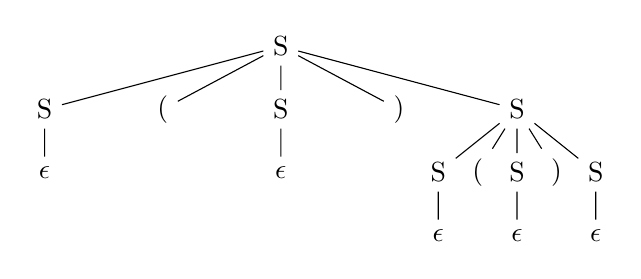
\begin{tikzpicture}[level 1/.style={level distance=8mm, sibling distance=15mm},
                    level 2/.style={level distance=8mm, sibling distance=5mm}]
  \node {S}
    child { node {S}
      child { node {$\epsilon$} }
    }
    child { node {(} }
    child { node {S}
      child { node {$\epsilon$} }
    }
    child { node {)} }
    child { node {S}
      child { node {S}
      child { node {$\epsilon$} }
      }
      child { node {(} }
      child { node {S}
      child { node {$\epsilon$} }
      }
      child { node {)} }
      child { node {S}
        child { node {$\epsilon$} }
      }
    }
  ;
\end{tikzpicture}
\newline
\newline
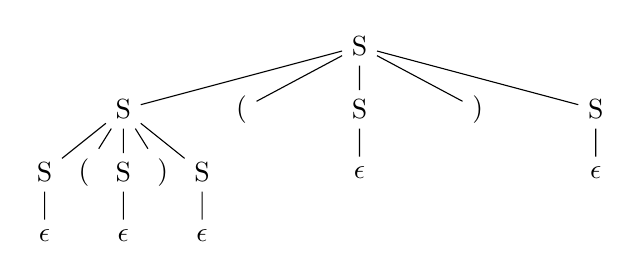
\begin{tikzpicture}[level 1/.style={level distance=8mm, sibling distance=15mm},
                    level 2/.style={level distance=8mm, sibling distance=5mm}]
  \node {S}
    child { node {S}
      child { node {S}
      child { node {$\epsilon$} }
      }
      child { node {(} }
      child { node {S}
      child { node {$\epsilon$} }
      }
      child { node {)} }
      child { node {S}
        child { node {$\epsilon$} }
      }
    }
    child { node {(} }
    child { node {S}
      child { node {$\epsilon$} }
    }
    child { node {)} }
    child { node {S}
      child { node {$\epsilon$} }
    }
  ;
\end{tikzpicture}
\end{document}
